\section{Experimental results}
\label{sec:results}
\subsection{Does the local bank improve the primary comparator?}
Table~\ref{tab:primary} reports the universal primary cohort of 58 targets. The comparator retains the same peer branch but uses a single mean of seven local detector evidences. At nominal $\alpha=0.01$, replacing that local branch with PACE raises mean detection from 0.807318 to 0.833405 at 100 local fitting rows and from 0.810681 to 0.838987 at 400 rows. The paired gains are 0.026086 and 0.028306. At $\alpha=0.05$, the corresponding gains are 0.023418 and 0.023219. All four corpus-stratified bootstrap intervals exclude zero.

These are absolute differences in target-macro detection rate, not relative percentage improvements or estimates of packet-weighted operational detection. The intervals describe resampling of the observed target differences within the available corpus strata. They do not incorporate uncertainty from choosing new corpora or from cohort selection.

\begin{table}[tb]
\centering\small
\caption{Universal primary comparison with the mean-ensemble local branch, 58 targets. Intervals are 95\% corpus-stratified paired bootstrap intervals. Detection rates are averaged over attack types, learning seeds, and targets.}
\label{tab:primary}
\begin{tabular}{rrrrl}
\toprule
$\alpha$ & $N$ & PACE & Comparator & Gain [95\% interval]\\
\midrule
0.01 & 100 & 0.833405 & 0.807318 & 0.026086 [0.011323, 0.043346]\\
0.01 & 400 & 0.838987 & 0.810681 & 0.028306 [0.012339, 0.047375]\\
0.05 & 100 & 0.894767 & 0.871348 & 0.023418 [0.005777, 0.043968]\\
0.05 & 400 & 0.896837 & 0.873619 & 0.023219 [0.003116, 0.045968]\\
\bottomrule
\end{tabular}

\end{table}

The nominal comparison is not a comparison at equal realized false-alert rates. At $\alpha=0.01$, PACE increases the mean false-alert rate by 0.003476 at 100 rows and 0.001588 at 400 rows. At $\alpha=0.05$, it reduces it by 0.001984 and 0.010070. Thus the detection gains at the smaller nominal operating parameter partly accompany increased benign alerts. At the larger parameter, the mean detection and mean false-alert differences both favor PACE, although averages alone do not establish dominance for individual targets.

\subsection{How much remains after operating-point adjustment?}
The stored budget sweep yields primary comparator-adjusted gains of 0.024659, 0.025735, 0.022176, and 0.020718 for the four settings in Table~\ref{tab:primary}. The four intervals, in the same order, are $[0.009682,0.042034]$, $[0.009690,0.044983]$, $[0.005135,0.042086]$, and $[0.002056,0.042482]$. These estimates remain positive, but their interpretation requires the actual interpolation procedure.

For each target and learning seed, the reporting code sorts PACE's four sweep points by realized benign false-alert rate and linearly interpolates detection at the comparator's rate. When that rate falls outside the observed sweep, the calculation uses the nearest endpoint. It then averages the resulting differences over seeds and targets. Consequently, these figures are clamped sweep-adjusted comparisons, not evidence that every detector was evaluated at precisely the same false-alert rate. The primary calculation also differs from a separate max-fusion reporting routine that constructs a monotone envelope and rejects uncovered operating points. Claims about primary matched comparisons must use the former definition. The narrow four-point sweep and endpoint handling limit how much this analysis can resolve operating-point confounding. Of 174 target--seed cells per setting, the comparator rate falls below or above the PACE sweep in 47/28 cells at $\alpha=0.01$, $N=100$, and 49/20 cells at $N=400$. At $\alpha=0.05$, these counts are 12/24 and 9/19. Thus 75, 69, 36, and 28 comparisons respectively use endpoints outside the covered range. These counts are derived from the stored campaign sweeps; they make explicit how often the reported adjustment cannot actually match the comparator rate.

\subsection{Are false alerts compatible with the nominal parameter?}
Table~\ref{tab:fpr} gives the distribution of target false-alert rates after averaging over learning seeds. At $\alpha=0.01$, PACE's mean is 0.033992 at 100 rows and 0.032369 at 400 rows, while the medians are 0.006485 and 0.006419. The large difference between means and medians indicates substantial heterogeneity. The worst target averages are 0.669005 and 0.670842. About 26\% of targets exceed twice the nominal parameter in both settings. A nominal value of 0.01 therefore cannot be interpreted as a one-percent test-time false-alert bound.

\begin{table}[tb]
\centering\small
\caption{Distribution of PACE's target-level realized false-alert rates, averaged over three learning seeds. Exceedance columns are proportions of targets, not proportions of individual benign rows or target--seed cells.}
\label{tab:fpr}
\begin{tabular}{rrrrrrrr}
\toprule
$\alpha$ & $N$ & Mean & Median & 90th pct. & Worst & $>\alpha$ & $>2\alpha$\\
\midrule
0.01 & 100 & .033992 & .006485 & .062058 & .669005 & .413793 & .258621\\
0.01 & 400 & .032369 & .006419 & .067903 & .670842 & .396552 & .258621\\
0.05 & 100 & .055453 & .019118 & .162115 & .671844 & .224138 & .137931\\
0.05 & 400 & .054337 & .018427 & .159692 & .671844 & .241379 & .137931\\
\bottomrule
\end{tabular}

\end{table}

The comparator has the same qualitative failure: at $\alpha=0.01$, its mean rates are 0.030516 and 0.030781, and its worst-target rates are 0.670174 and 0.670842. This shared failure does not excuse PACE's additional alerts. It shows that calibration on earlier benign data is insufficient to deliver the nominal rate on the later benign role in this benchmark. The results alone cannot assign the discrepancy to a unique cause, such as temporal shift, sample selection, or score extrapolation. Moreover, the resolution rule's allocation sum already exceeds 0.01 before considering any test-distribution change.

At $\alpha=0.05$, PACE's means are 0.055453 and 0.054337; the corresponding 90th percentiles are 0.162115 and 0.159692. The worst value remains 0.671844. Even where the pooled average approaches the nominal parameter, the upper tail is unsuitable evidence for uniform operational control. A row-level false-alert rate is also not an incident-level alert burden: aggregation, duplicate suppression, analyst capacity, and the benign-to-attack prevalence of a deployed stream were not measured.

Figure~\ref{fig:false-alerts} shows the complete cumulative distributions, including the long upper tails that are obscured by pooled means.
\begin{figure}[p]
\centering
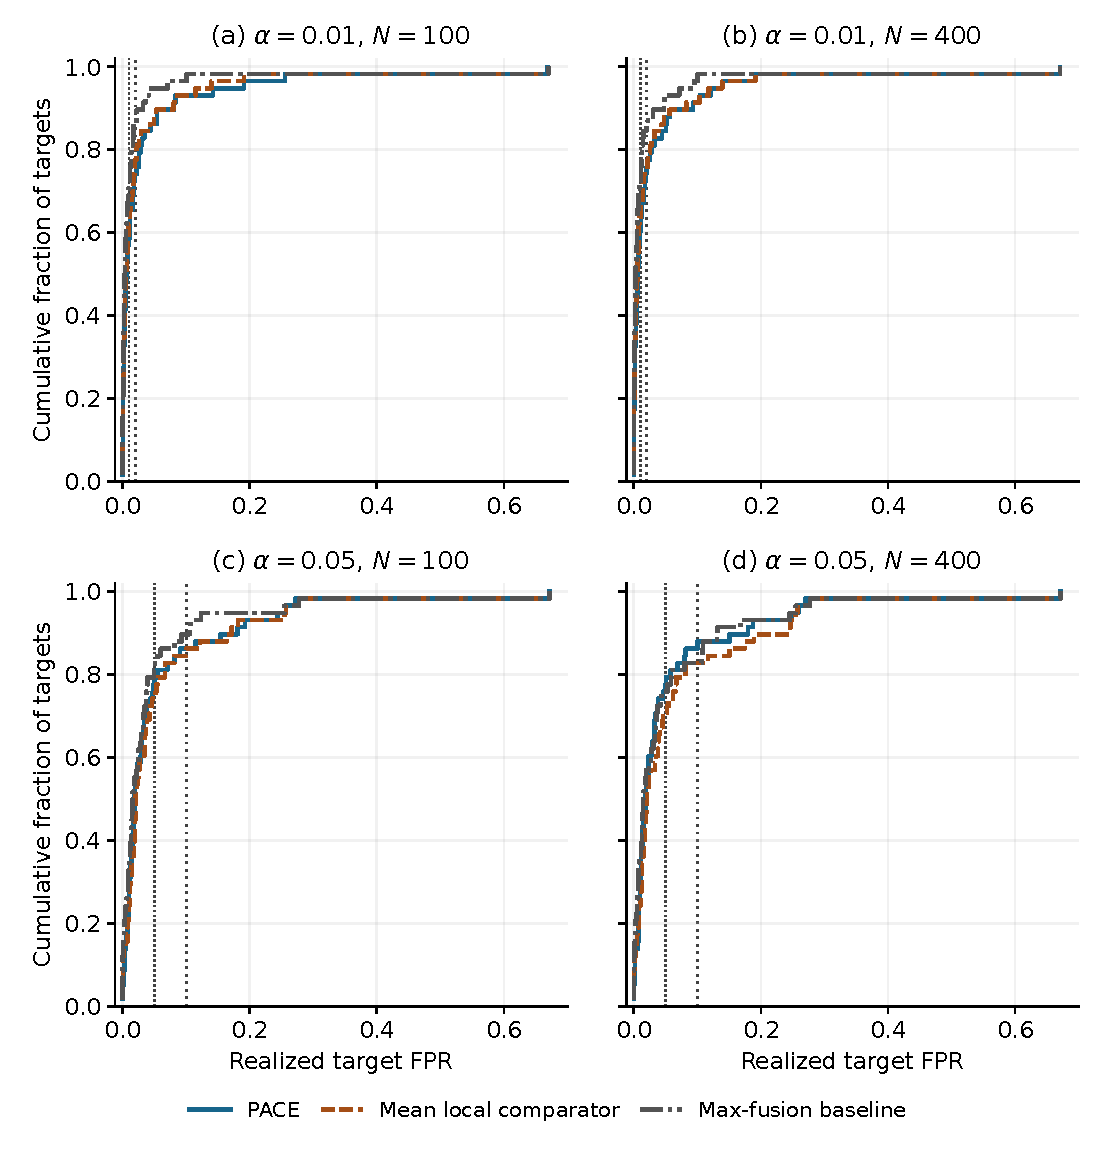
\includegraphics[width=\textwidth]{figures/false-alert-distribution.pdf}
\caption{Empirical cumulative distributions of benign test false-alert rates for 58 targets, after averaging each target over three learning seeds. Dashed vertical guides mark $\alpha$ and $2\alpha$; they are nominal reference values, not demonstrated bounds. The recorded max-fusion baseline includes the mean-ensemble local branch. Curves reproduce the frozen figure unchanged; color distinguishes methods, while Table~\ref{tab:fpr} supplies numerical PACE distribution summaries independently of color.}
\label{fig:false-alerts}
\end{figure}
\subsection{Where are the gains concentrated?}
TON\_IoT has the largest stratum mean gains: 0.117448 and 0.126729 at $\alpha=0.01$, and 0.120780 and 0.104447 at $\alpha=0.05$, for 100 and 400 fitting rows respectively. Removing its nine targets reduces the pooled gains to 0.009306, 0.010228, 0.005536, and 0.008299. Their intervals are $[0.001808,0.019526]$, $[0.000995,0.024240]$, $[0.000090,0.014343]$, and $[0.000143,0.022250]$. The remaining gains are positive in these primary summaries but small, and two lower bounds lie very close to zero.

N-BaIoT is already near complete detection and changes by approximately $10^{-5}$ or less. Gotham gains range from 0.001950 to 0.005907. UNSW G2 improves by 0.009251 and 0.005548 at $\alpha=0.01$, but changes by $-0.001420$ and $-0.002037$ at $\alpha=0.05$. Several stratum intervals include zero. The median target gain is zero in many strata, so a positive mean should not be paraphrased as an improvement for most devices.

IoT-23's primary mean gains range from 0.017582 to 0.029670, but its target-level pattern is concentrated rather than uniform. At $\alpha=0.01$ and 400 rows, CTU-13's mean gain is 0.003156 with interval $[-0.007871,0.017066]$. Scenario 12 loses 0.032595, the only primary target loss exceeding 0.01. No primary target loses more than 0.05. The comparator's autoencoder and PACE's different anchor composition are possible contributors to this regression; the final ablation set does not isolate a causal attribution to the autoencoder alone.

Figure~\ref{fig:targets} displays the concentration of the gains and the negative tail without aggregating targets into stratum means.
\begin{figure}[p]
\centering
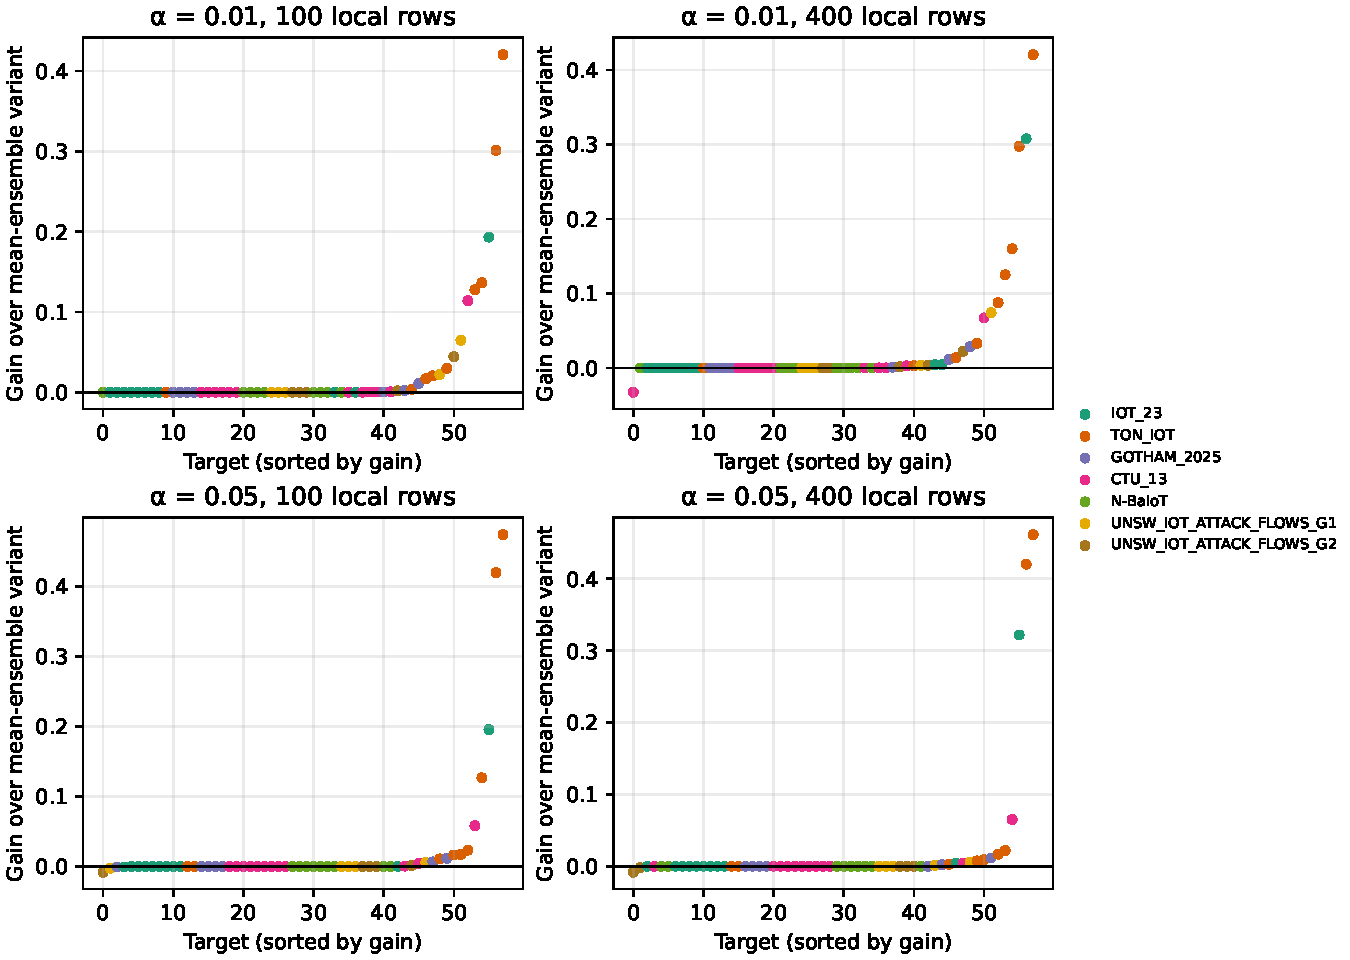
\includegraphics[width=\textwidth]{figures/target-gains.pdf}
\caption{Target-level detection differences, PACE minus the mean-ensemble local comparator. Each panel independently sorts its 58 seed-averaged target differences; a horizontal position is a rank, not a shared target identity across panels. Colors identify study strata. The overall concentration and negative differences remain visible in grayscale; stratum attribution requires the legend colors and is described numerically in the text. Axes report absolute detection-rate differences, not percentages.}
\label{fig:targets}
\end{figure}
\subsection{Which components supply complementary detections?}
Removing the rarity family costs 0.008626 and 0.011977 in pooled detection at $\alpha=0.01$, compared with 0.003413 and 0.002013 for removing feature experts, and 0.002008 and 0.002796 for removing the response expert. At $\alpha=0.05$, the rarity costs remain 0.006020 and 0.010403; feature costs are only 0.000127 and 0.000344. The response expert's costs are 0.003118 and 0.001269. These results support a modest complementary contribution, especially from rarity, rather than identifying response-space modeling as the main source of the improvement.

Ablation changes also recalibrate the remaining union. They are not additive decompositions of the gain and cannot be summed to assign causal importance. Replacing target-relative peer responses by raw margins changes pooled detection by only 0.001101--0.002879 across primary settings. Several corresponding intervals include zero. The evidence for the particular response representation is therefore weaker than the overall comparison with the mean-ensemble local branch.

The anchor has a tradeoff. Removing it reduces mean detection at $\alpha=0.01$, but the corresponding intervals include zero. At $\alpha=0.05$, the bank without the anchor detects more: its rates are 0.897598 and 0.898372, versus PACE's 0.894767 and 0.896837. Its false-alert rates are also higher, at 0.060458 and 0.064650. A single local union gives identical detection to PACE at $\alpha=0.01$ to the precision of the stored table; at $\alpha=0.05$ its differences are small and its false-alert rates higher. These outcomes do not establish that the tier structure is uniformly superior.

Within the final PACE rule, the attack-detection decomposition distinguishes alerts unique to the local branch from detections shared with peers. At $\alpha=0.01$ and 400 rows, local-exclusive detection is 0.147434 in TON\_IoT and 0.120957 in IoT-23, but only 0.000042 in N-BaIoT. These quantities are coverage fractions within the final rule, not gains over the mean-ensemble comparator and not the performance of a separately calibrated local-only detector.

\subsection{Does more local fitting data reliably help?}
On the same 58 targets, increasing the fitting budget from 100 to 400 rows changes PACE detection by 0.005582 at $\alpha=0.01$, with interval $[-0.003760,0.015387]$, and by 0.002070 at $\alpha=0.05$, with interval $[-0.004456,0.008690]$. Neither interval excludes zero. The local branch alone gains much more coverage, but much of that coverage overlaps detections already supplied by peers. The combined rule need not improve proportionally to the local branch.

At 750 rows, the universal cohort retains gains over the comparator of 0.024276 and 0.022614. However, at $\alpha=0.05$, the interval for the gain excluding TON\_IoT includes zero. The 2000-row analysis contains only the 47 targets with enough training-role observations. Its gains over the comparator are 0.019624 and 0.007358; both sweep-adjusted intervals include zero. At $\alpha=0.05$, the gain excluding TON\_IoT is negative, $-0.000370$, with interval $[-0.000712,-0.000074]$.

The 20,000-row cohort contains 15 targets. Its nominal gains are 0.005329 at $\alpha=0.01$ and $-0.001311$ at $\alpha=0.05$, with intervals including zero. Within this cohort, increasing the budget from 100 to 20,000 rows at $\alpha=0.05$ reduces PACE detection by 0.028296, with interval $[-0.032827,-0.023766]$. The results therefore do not support monotonic improvement with additional local fitting data. Comparisons across the 58-, 47-, and 15-target cohorts would confound fitting budget with target composition and are not used as estimates of budget effects.

Figure~\ref{fig:budgets} summarizes comparator gains within each fixed resource-eligible cohort.
\begin{figure}[tbp]
\centering
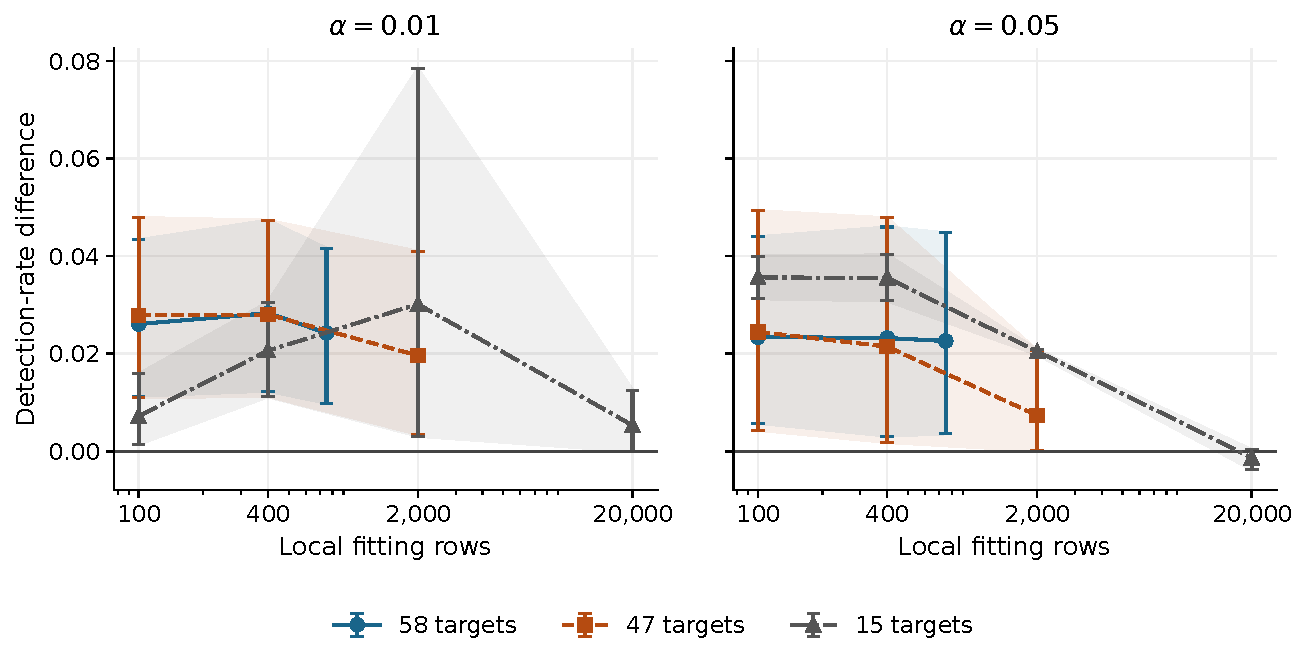
\includegraphics[width=\textwidth]{figures/budget-scaling.pdf}
\caption{Detection gain over the mean-ensemble local comparator as a function of local fitting rows on a logarithmic horizontal axis. The universal primary and robustness cohorts contain the same 58 targets; their curves overlap at shared budgets. Broad scaling uses 47 targets and the plotted ``extreme high-resource'' analysis uses 15. Shading gives 95\% corpus-stratified bootstrap intervals at evaluated budgets; connecting lines and bands are visual guides, not additional experiments. Compare budgets within a curve; differences between curves also reflect cohort composition. Color identifies cohorts; numerical findings in the text give the principal trends independently of color.}
\label{fig:budgets}
\end{figure}
\subsection{Seed stability and engineering acceptance}
Every learning seed has a positive primary pooled gain, ranging from 0.015977 to 0.039551 across settings. This consistency is narrower than generalization to new targets: all three seeds reuse the same data and splits. Excluding TON\_IoT, seed 6 has a gain of $-0.000195$ at $\alpha=0.05$ and 400 rows. Every primary leave-one-study-stratum-out pooled gain is positive, but this sensitivity check still operates on the same collection of corpora and targets.

The primary cells satisfy the repository's engineering acceptance criteria, which permit a limited fraction of harmed targets, bound changes in realized false alerts, and require positive aggregate summaries. This is not a formal statistical non-inferiority test or independent external validation. In particular, the observed scenario-12 regression remains a regression despite satisfying the aggregate acceptance rule. The larger-budget non-gating analyses contain failures of individual criteria and are reported as such, rather than being used to extend the primary verdict.



